This chapter presents the results of the conducted experiments. First, an overview of the results achieved with the entire system is provided. Subsequently, individual components of the system are examined in more detail.
The code and documentation are made publicly available. Further information can be found in \chref{online_sources}.

\section{Entire System}
%
\begin{figure}[h]
    \centering
    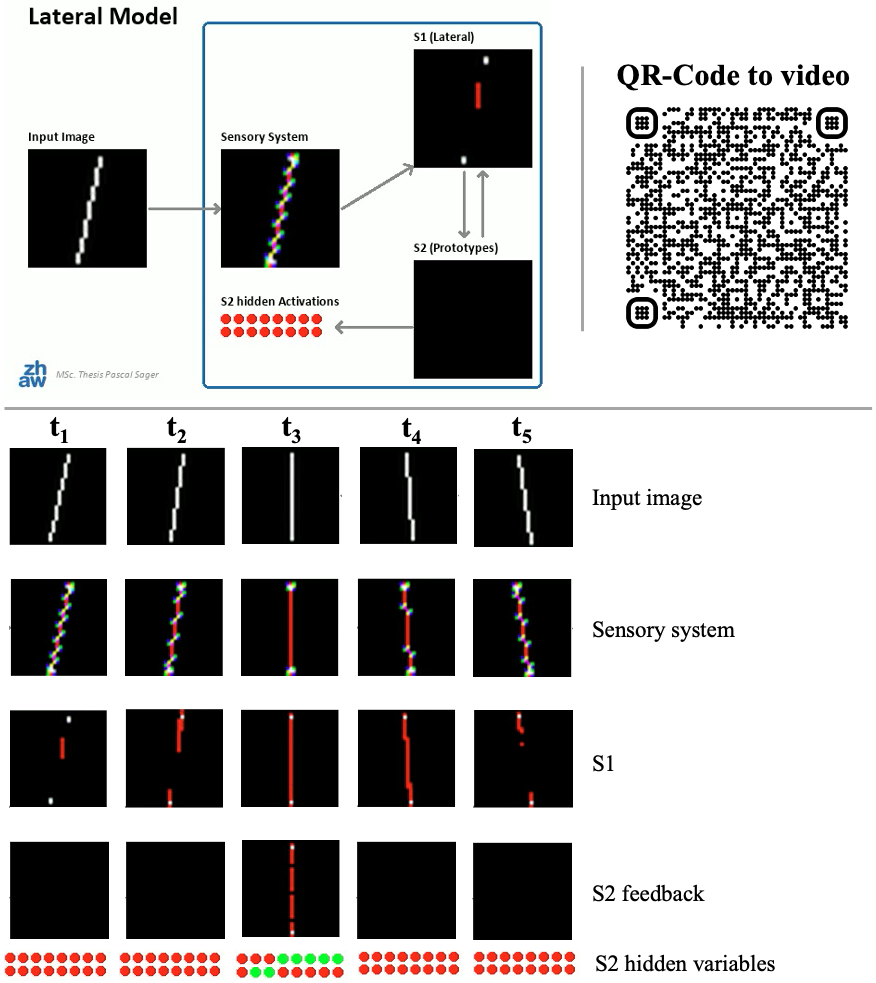
\includegraphics[width=0.99\textwidth]{r1_overview}
    \caption[Frames of a video visualising the model's activations]{Frames of a video visualising the model's activations. At the top of the image, an actual video frame and a QR code linking to the video are shown. At the bottom of the image, the changing network activations over time are visualised.}
    \figlbl{r1_overview}
\end{figure}
%
An overview of the entire system is provided in \figref{r1_overview}.
This image is derived from a video available online at \href{https://sagerpascal.github.io/lateral-connections/results/final_results.html#video-visualisations}{sagerpascal.github.io/lateral-connections} or with the QR code on the top right of the figure.
For a detailed explanation of the components shown in the video, please refer to \secref{result_video}.
The video shows the network's activations for a straight line rotated counterclockwise around its centre.
In the lower part of \figref{r1_overview}, a series of five network states is shown shortly before and after a vertical line is reached.

The network has only been trained on vertical, horizontal, and diagonal lines.
Therefore, many lines fed into the network in this video represent unknown objects.
However, \emph{S1} still detect some learned patterns, such as multiple pixels aligned vertically, horizontally, or diagonally.
Therefore, it can provide lateral support between local pixel groups representing such a pattern.
The closer the input becomes to a learned pattern, the bigger the lateral support.
At time $t_3$, the input corresponds to a vertical line as observed during training.
In that case, all pixels receive enough lateral support to remain active.

For the conducted experiments, \emph{S2} does not map the net fragments to a reference frame but acts as a memory of learned objects.
As long as the net fragments represent an unknown pattern, no latent cells in \emph{S2} are activated and no feedback to \emph{S1} is provided.
However, when the net fragments in \emph{S1} correspond to a learned pattern, \emph{S2} provides feedback and further increases certainty in \emph{S1}.
When replacing the memory used to simulate \emph{S2} with projection fibres, the feedback should be even better, as \emph{S2} will be able to detect transformed objects.

Overall, the network's behaviour is as expected: \emph{S1} builds net fragments based on well-known patterns observed during training.
However, images not seen during training also contain local patterns similar to those from the training data and, therefore, still receive local support through lateral connections.
\emph{S2} responds to patterns stored in its memory, only providing support to \emph{S1} for objects seen during training.

Furthermore, all samples seen during training have automatically been saved in \emph{S2}.
The system is able to produce net fragments that roughly reassemble the input from the sensory system.
However, the net fragments are more robust than the sensory system, as shown in the following sections.

\subsection{Effect of Noise}
%
\begin{figure}[h]
    \centering
    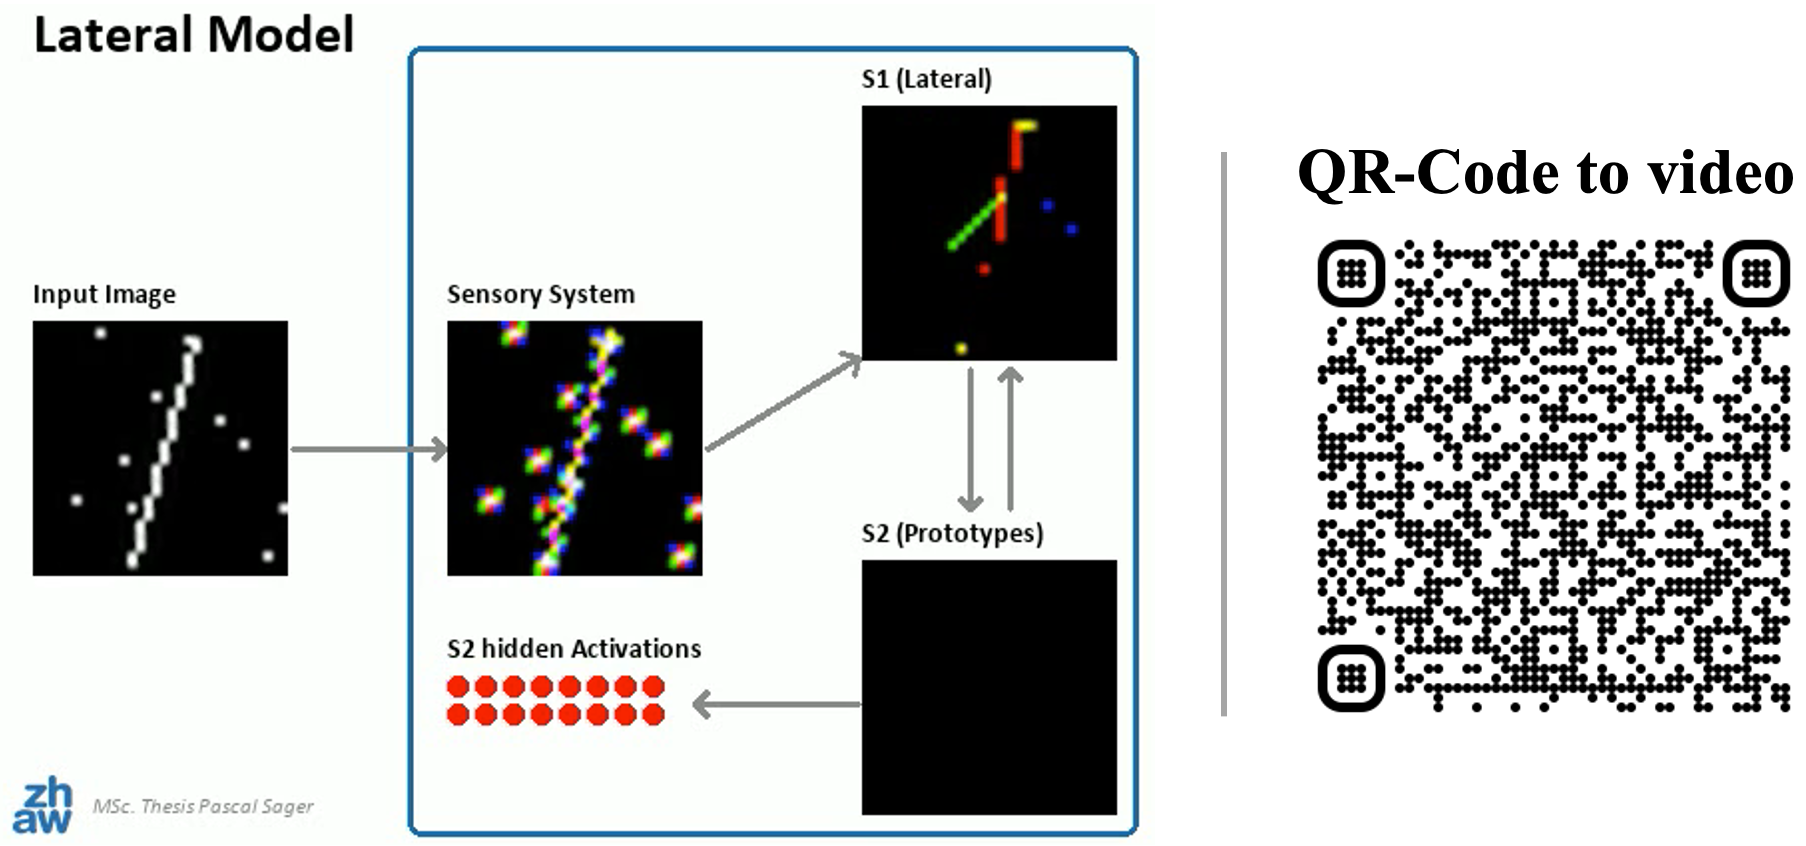
\includegraphics[width=0.99\textwidth]{r2_overview}
    \caption[Video visualising the network's behaviour with noise in input]{A frame of a video visualising the network's behaviour if noise is added to the data. The QR code on the right links to the corresponding video.}
    \figlbl{r2_overview}
\end{figure}
%
\figref{r2_overview} refers to a video demonstrating the network's behaviour when noise is added to the input data.
The noise is generated by randomly flipping a pixel in the input data from $0$ to $1$ or vice versa with a probability of $0.005$.

To assess the network's ability to deal with noise, the same input is fed into the model twice: once with noise and once without. The activations of \emph{S1} for these two versions of the input image are compared, and the percentage of feature cells that are initially triggered by the introduced noise but subsequently deactivated due to insufficient support is measured.

This analysis shows that the system can remove about $71.2\%$ of the noise from the input data. However, this effectiveness is mainly due to the fact that a single noise pixel triggers $3$ cells in each feature channel of the sensory system, resulting in $12$ active cells. After building net fragments, only the four feature cells in the centre of this cluster remain active, giving the impression that the noise has been removed while, in reality, it only has been reduced.

\begin{figure}[h]
    \centering
    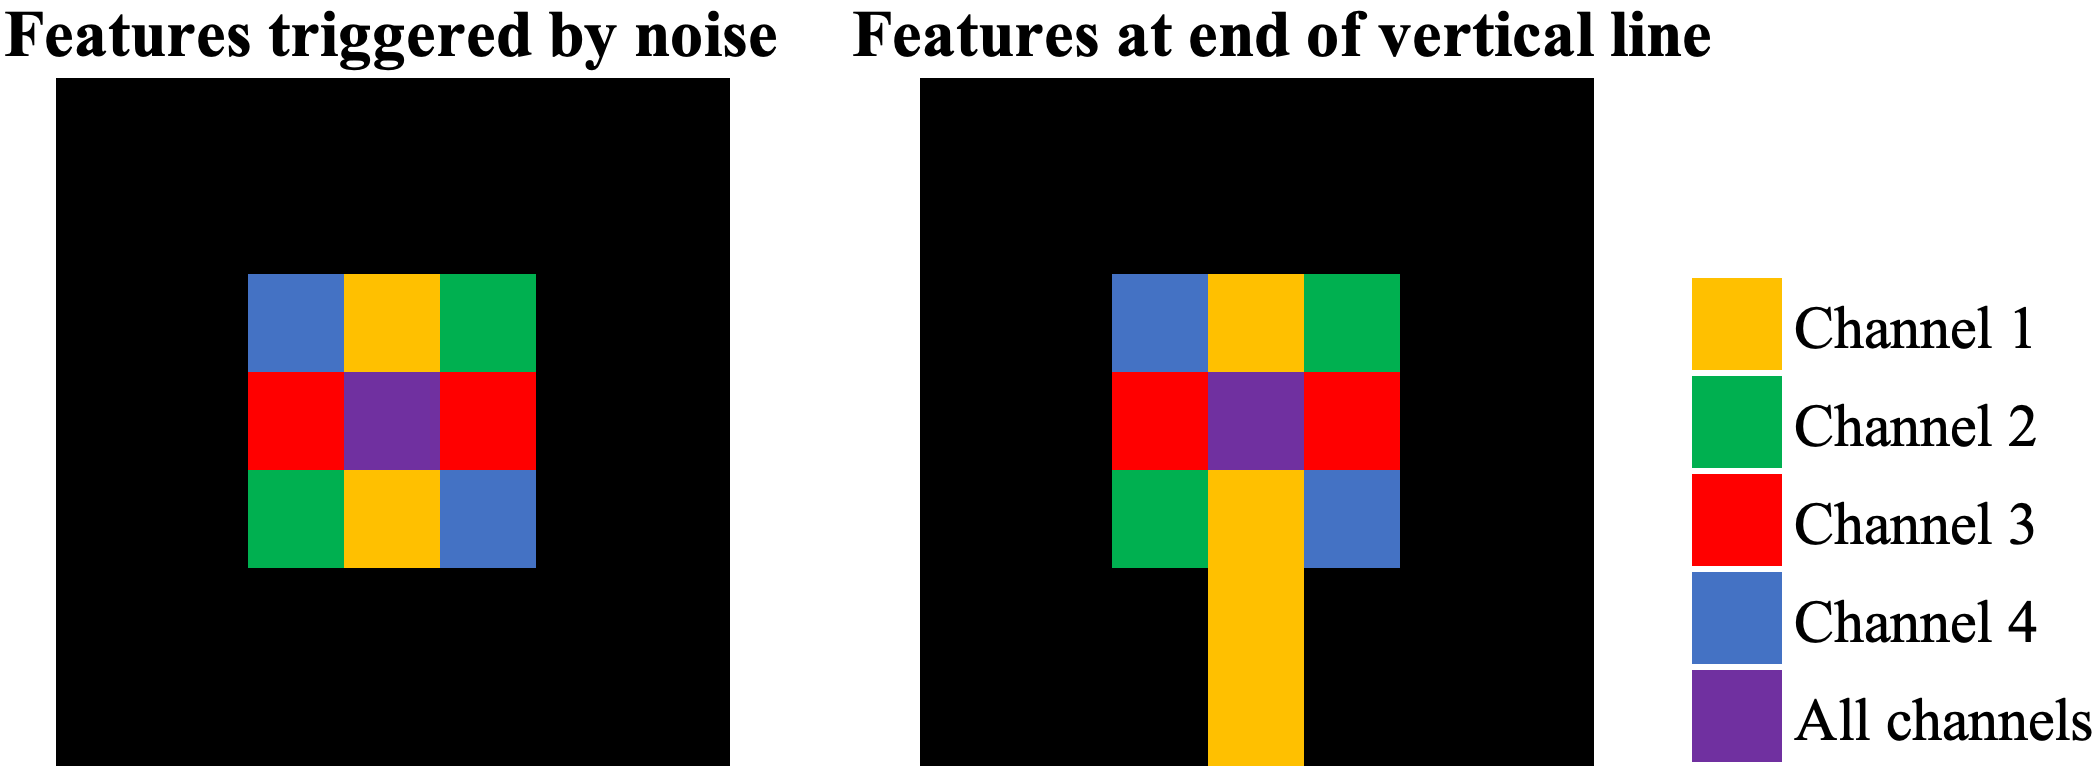
\includegraphics[width=0.49\textwidth]{features_noise_data}
    \caption[Features triggered by noise]{The features triggered by noise (on the left) compared with the features triggered by a line end (on the right).}
    \figlbl{features_noise_data}
\end{figure}
%
In fact, only in $23.8\%$ of the cases is noise in the input completely removed.
Several reasons contribute to the difficulty of obliterating noise: First, noise can be located close to the line or other noise and thus receives lateral support from other cells. Second, when observing noise in the input, the sensory system triggers activations in all feature channels similar to activations found at line ends as visualised in \figref{features_noise_data}.
As a result, activations triggered by noise correspond to a well-known pattern. Therefore, these cells support each other and cannot be adequately filtered by the system.
Overall, this behaviour is to be expected, and noise should only be filtered out if it is significantly different from learned patterns.

Although the noise cannot be completely filtered out, the net fragments are still accurately mapped to the correct prototype in \emph{S2}. Thus, the system still correctly interprets the input despite the noise.

\subsubsection{Noise per Channel}
%
\begin{figure}[h]
    \centering
    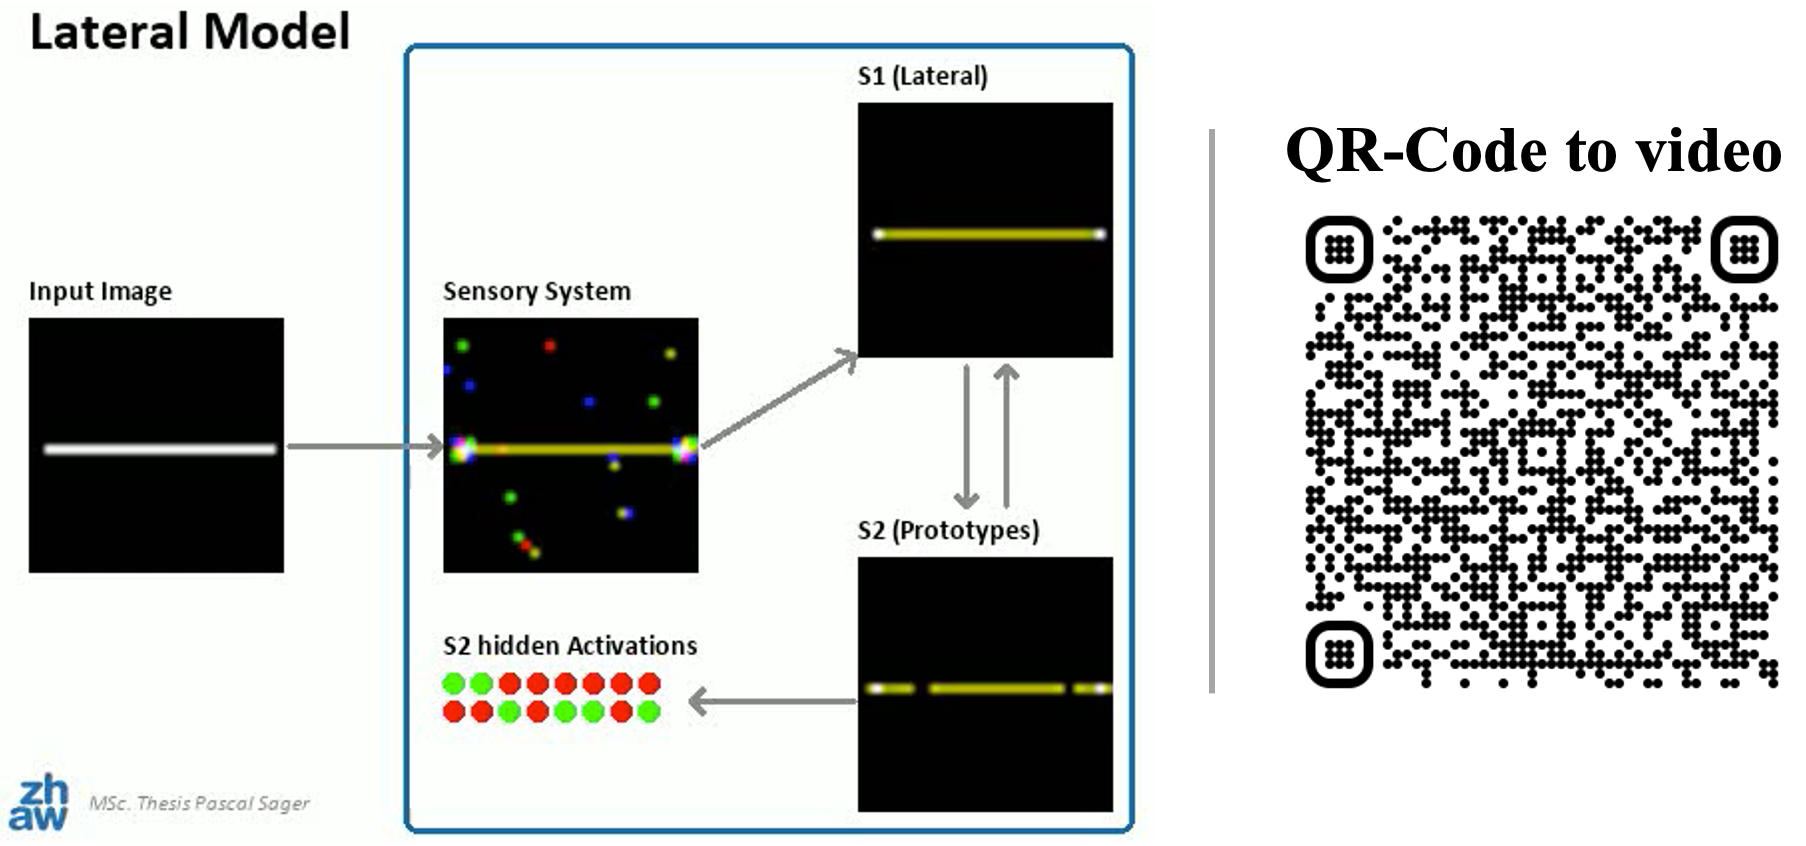
\includegraphics[width=0.99\textwidth]{r3_overview}
    \caption[Video visualising the network's behaviour with noise in the feature channels]{A frame of a video visualising the network's behaviour if noise is added to the feature channels. The QR code on the right links to the corresponding video.}
    \figlbl{r3_overview}
\end{figure}
%
In this section, it is investigated whether noise can be filtered when there is no correlation between the locations of the noise within the feature channels.
Thus, the noise does not correspond to learned patterns anymore.
Therefore, noise is not added to the input data but to each feature channel of the sensory systems' output separately.
This experiment is considered more relevant for real-world scenarios, as future systems that deal with real-world data will have a much larger number of input channels and more diverse patterns, making it unlikely that noise resembles a learned pattern that the network considers valid.

\figref{r3_overview} refers to a video demonstrating the networks' behaviour when noise is added to each feature cell with a probability of $0.005$.
In this case, about $91.7\%$ of the noise is removed, demonstrating the network's high robustness to such perturbations.
The noise that is not removed is the noise that is very close to the actual line and therefore receives support from a valid object.

\subsection{Discontinuous Line}
%
\begin{figure}[h]
    \centering
    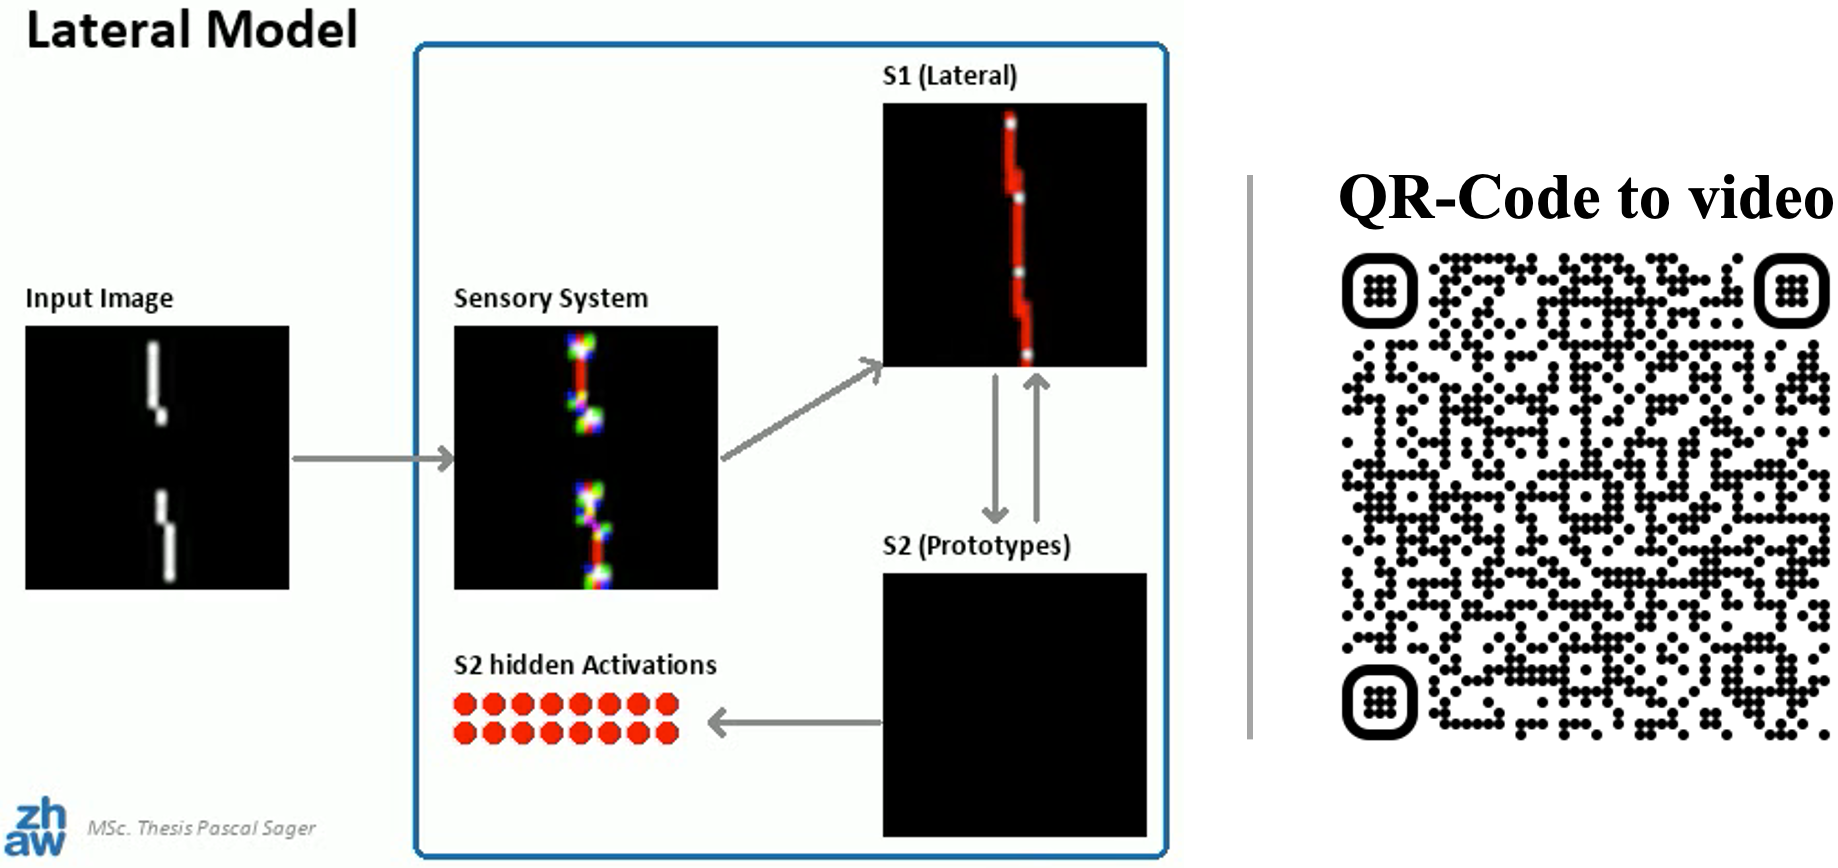
\includegraphics[width=0.99\textwidth]{r4_overview}
    \caption[Video visualising the network's behaviour for discontinuous lines]{A frame of a video visualising the network's behaviour for discontinuous lines. The QR code on the right links to the corresponding video.}
    \figlbl{r4_overview}
\end{figure}
%
Lateral connections can not only reduce noise but also recreate occluded objects.
This phenomenon is demonstrated by analysing the network's behaviour if a discontinuous line is fed into the network.
\figref{r4_overview} contains a QR code linking to a video demonstrating that \emph{S1} is able to reconstruct lines that are interrupted by up to $8$ pixels.

In the experimental setup, the centre of the line is detected, and a varying number of pixels starting from the centre are intentionally switched off.
The feedback from \emph{S2} is switched off so that only the reconstruction based on net fragments within \emph{S1} is tested.
Remarkably, the \emph{S1} consistently succeeds in reconstructing the original training input when up to $6$ pixels are removed. Furthermore, in many cases, it can reconstruct lines with up to $8$ pixels missing, although it fails with more than $8$ pixels removed.

The extent to which the network can reconstruct discontinuous lines depends on the range of lateral connections $n_l$. As expected, increasing the value of $n_l$ allows \emph{S1} to reconstruct lines with more missing pixels, improving its performance in recovering objects.
However, $n_l$ should not be too large so that \emph{S1} build net fragments based on local features (c.f. \secref{neuroscience_findings_net_fragments}).

In the conducted experiments, the lateral reach is set to $n_l=11$.
The impressive ability to reconstruct up to $8$ missing pixels with this setting suggests that recreating occluded patterns works effectively.


\subsection{S2 Feedback}\seclbl{results_s2_feedback}
So far, lines have been reconstructed based on net fragments and lateral support present in \emph{S1}.
In the following, feedback from \emph{S2} is additionally incorporated in \emph{S1}, and it is analysed if \emph{S1} can efficiently utilise it.
Please note that not all aspects from \emph{S2} are implemented, and it is a memory that returns stored net fragments if they are similar to an observation.
Therefore, it only works for the examples the network encountered during the training process.

\begin{figure}[h]
    \centering
    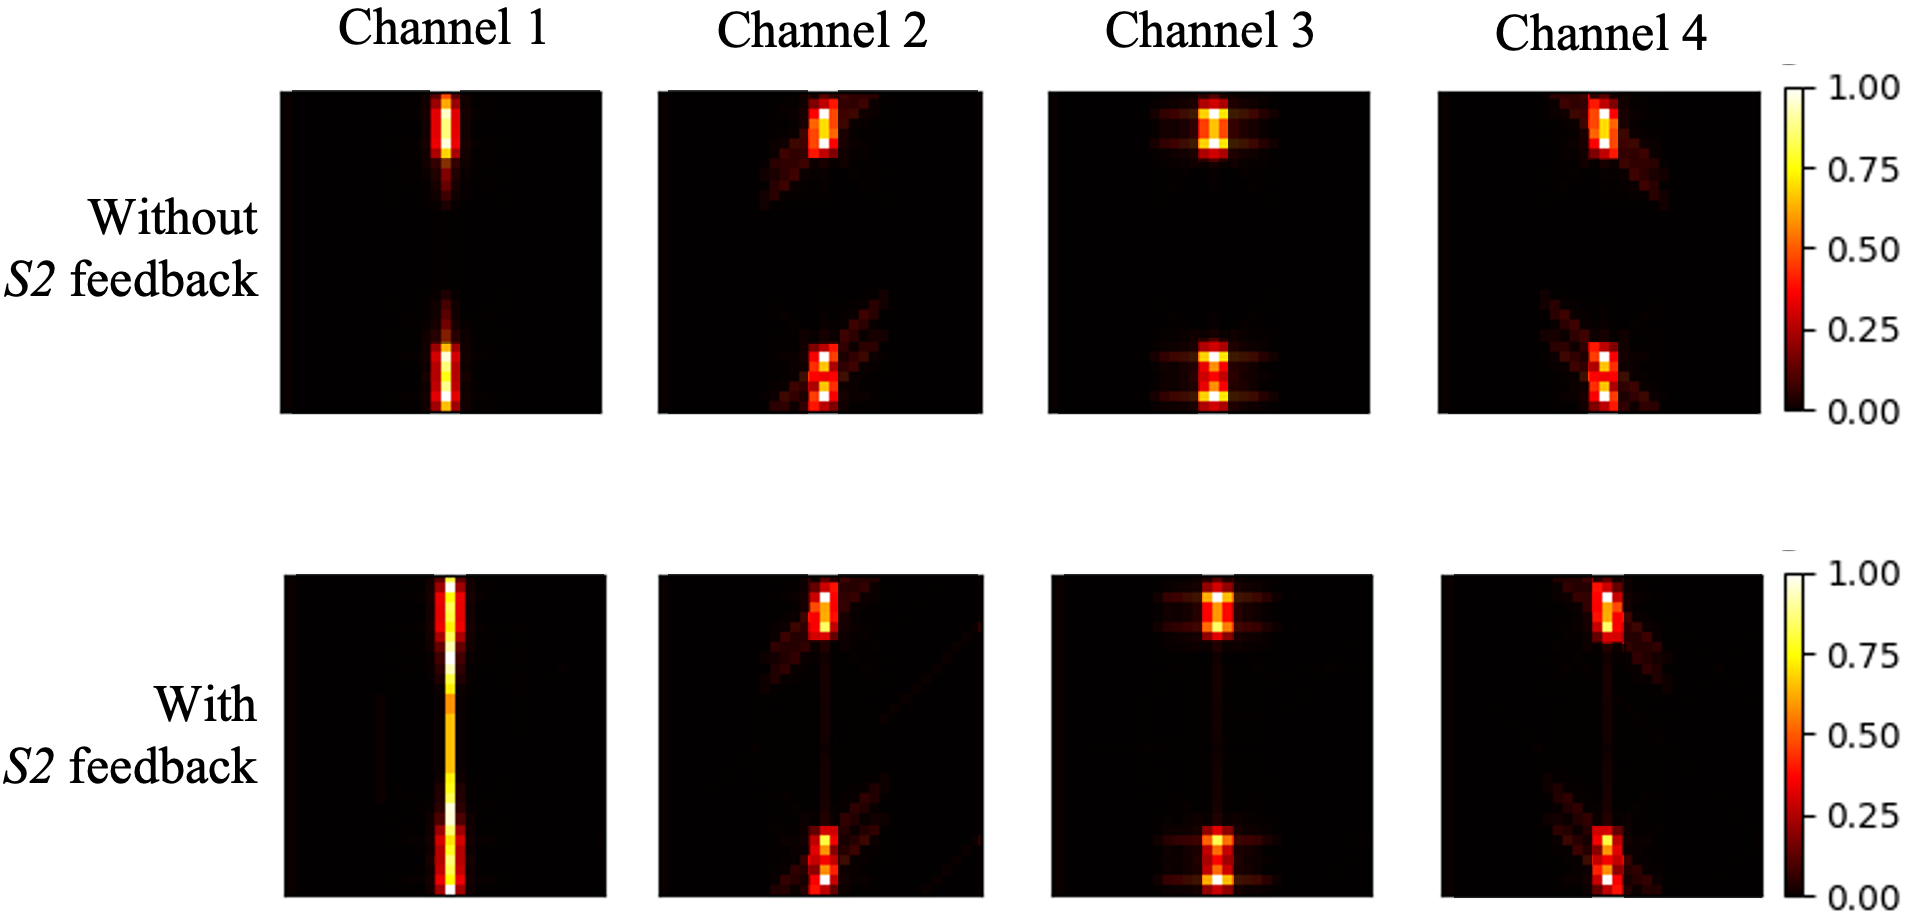
\includegraphics[width=0.99\textwidth]{s2_feedback_heatmap}
    \caption[Activation probabilities with/without \emph{S2} feedback]{The activation probabilities per cell across all four channels with and without feedback from \emph{S2}. The input is a discontinuous vertical line with $20$ pixels missing.}
    \figlbl{s2_feedback_heatmap}
\end{figure}
%
\figref{s2_feedback_heatmap} visualises the activation probabilities for all cells across the four output channels for a vertical line with $20$ missing pixels.
The top row shows the probabilities when no feedback form \emph{S2} is incorporated, and the bottom row the probabilities after the feedback is incorporated.

As visible in the top row of \figref{s2_feedback_heatmap}, without incorporating feedback from \emph{S2}, the line cannot be fully reconstructed using lateral connections in \emph{S1}, as $20$ of missing pixels exceeds the reach of lateral connections. However, \emph{S2} is still able to map the line with missing pixels to the correct prototype and provide appropriate feedback. After the feedback is incorporated, the activation probabilities for the entire vertical line increase significantly. Especially in the middle section, where the pixels have been removed, the activation probabilities increase from $0\%$ to approximately $65\%$.

When a continuous vertical line is fed into the system, the activation probability in the middle section of the line is above $90\%$.
This high probability aligns with the fact that the sensory signal and the memory's feedback are consistent.
However, when the memory expects activations that are not detected by the sensory system (e.g. due to the missing pixels), the activation probability decreases. This behaviour reflects meaningful modelling of the network's uncertainty when integrating feedback when occluded objects are encountered.

In conclusion, the feedback from \emph{S2} can be effectively incorporated into \emph{S1}.
It helps to deal with occluded objects and creates stability in net fragments, even when the sensory system does not detect (occluded) parts of the object.



\section{Model Weights}
%
\begin{figure}[h]
    \centering
    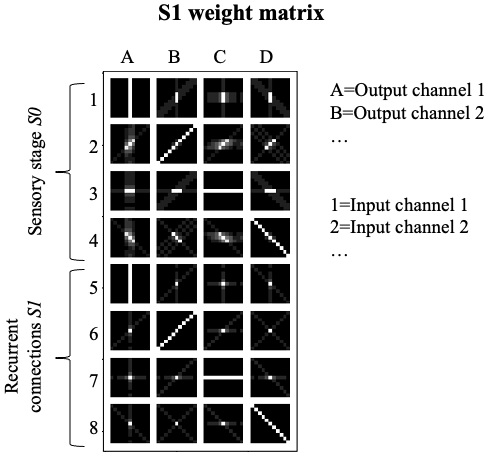
\includegraphics[width=0.79\textwidth]{S1_weight_matrix}
    \caption[Weight matrix of \emph{S1} after training]{The weight matrix of \emph{S1} after training.}
    \figlbl{S1_weight_matrix}
\end{figure}
%
The following section discusses the weight matrix of \emph{S1}, which contains the strength of the learned lateral connections.
\figref{S1_weight_matrix} visualises the learned weights. 
The input of \emph{S1} consists of four channels from the sensory stage (rows labelled as $1$-$4$) and four channels from recurrent connections (labelled as $5$-$8$).
\emph{S1} produces four output channels, and the kernels contributing to each output channel are depicted in columns labelled from $A$ to $D$.
Each output channel specialises in a different type of line: Output channel $A$ focuses on vertical lines, channel $B$ on diagonal lines with a positive slope, channel $C$ on horizontal lines, and channel $D$ on diagonal lines with a negative slope.

An analysis of output channel $A$, which focuses on horizontal lines, is presented in the following.
However, it is important to note that the four output channels have similar characteristics, with the main difference being that the filters are rotated by $45°$. Consequently, insights from channel $A$ are also transferable to all other channels.

\begin{figure}[h]
    \centering
    \includegraphics[width=0.99\textwidth]{S1_weight_analysis}
    \caption[Analysis of weight matrix]{An overview of the data processed by the weight matrix of \emph{S1}.}
    \figlbl{S1_weight_analysis}
\end{figure}
%
\figref{S1_weight_analysis} visualises the features processed when a horizontal line is fed into the system.
First, the sensory system extracts four features from the input (visualised in the box named ``output sensory system'').
Channel $1$ contains ``vertical-line features'', spanning the entire vertical length of the image. 
The channels $2$-$4$ contain features of diagonal and horizontal lines. However, the sensory system recognises these features only at the ends of the lines.
Thus, at the ends of the vertical line, about three neurons respond for each channel $2$-$4$ to represent these features.
These features extracted by the sensory system are fed into the channels $1$-$4$ of \emph{S1}.
As expected, these features have been incorporated into the weight matrix accordingly (see $A1$-$A4$).

Based on these features, output channel $A$ generates a response roughly corresponding to the vertical line originally fed into the system.
Thus, channel $A$ fulfils its purpose and represents vertical lines.
Besides channel $A$, also the channels $B$-$D$ become active.
However, these channels specialise in different lines and only activate exactly one pixel at the line ends, where the sensory system produces a very high activity across all channels.
Thus, many cells are active at the line end, supporting each other.

The output of \emph{S1} is reused as an input signal in the next timestep $t+1$.
This is implemented as a recurrent connection between the output channels $A$-$D$ and the input channels $5$-$8$.
As expected, the filters processing the recurrent input for output channel $A$ specialise in the activity that is produced by \emph{S1} for vertical lines:
When a vertical line is processed, the output channel $A$ produces a vertical line and the channels $B$-$D$ a single-cell activation, corresponding to the filters $A5$-$A8$.


\subsection{Weight Normalisation}
%
\begin{figure}[h]
    \centering
    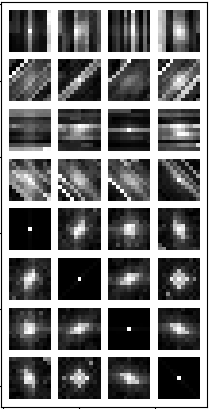
\includegraphics[width=0.35\textwidth]{weights_no_norm}
    \caption[Weights after training without normalisation]{Weight matrix of \emph{S1} after training without weight normalisation.}
    \figlbl{weights_no_norm}
\end{figure}
%
As described in \secref{framework_norm}, the weight is normalised in the range $0, ..., 1$.
Normalising the weights is crucial for the proper functioning of the network. Without weight normalisation, lateral support could be dominated by a single cell, resulting in infinite lateral support if trained long enough. In the human brain, there is no such dominance of single cells, and neighbouring cells play an equally important role in providing support \sidecite{kandel_principles_2013}.

After $10$ epochs without weight normalisation, some lateral connections reach a weight above $74$ and dominate the decision process of whether neighbouring cells should remain active.
This leads to undesired activations and weight updates. 
\figref{weights_no_norm} depicts the weight matrix after $10$ epochs if trained without weight normalisation.
No clear structure is visible within the weights, and the support provided within the network appears rather random. 
Thus, normalisation is not only biologically more plausible but also a necessity to obtain meaningful lateral weights.



\subsection{Initialisation}
\begin{figure}[h]
    \centering
    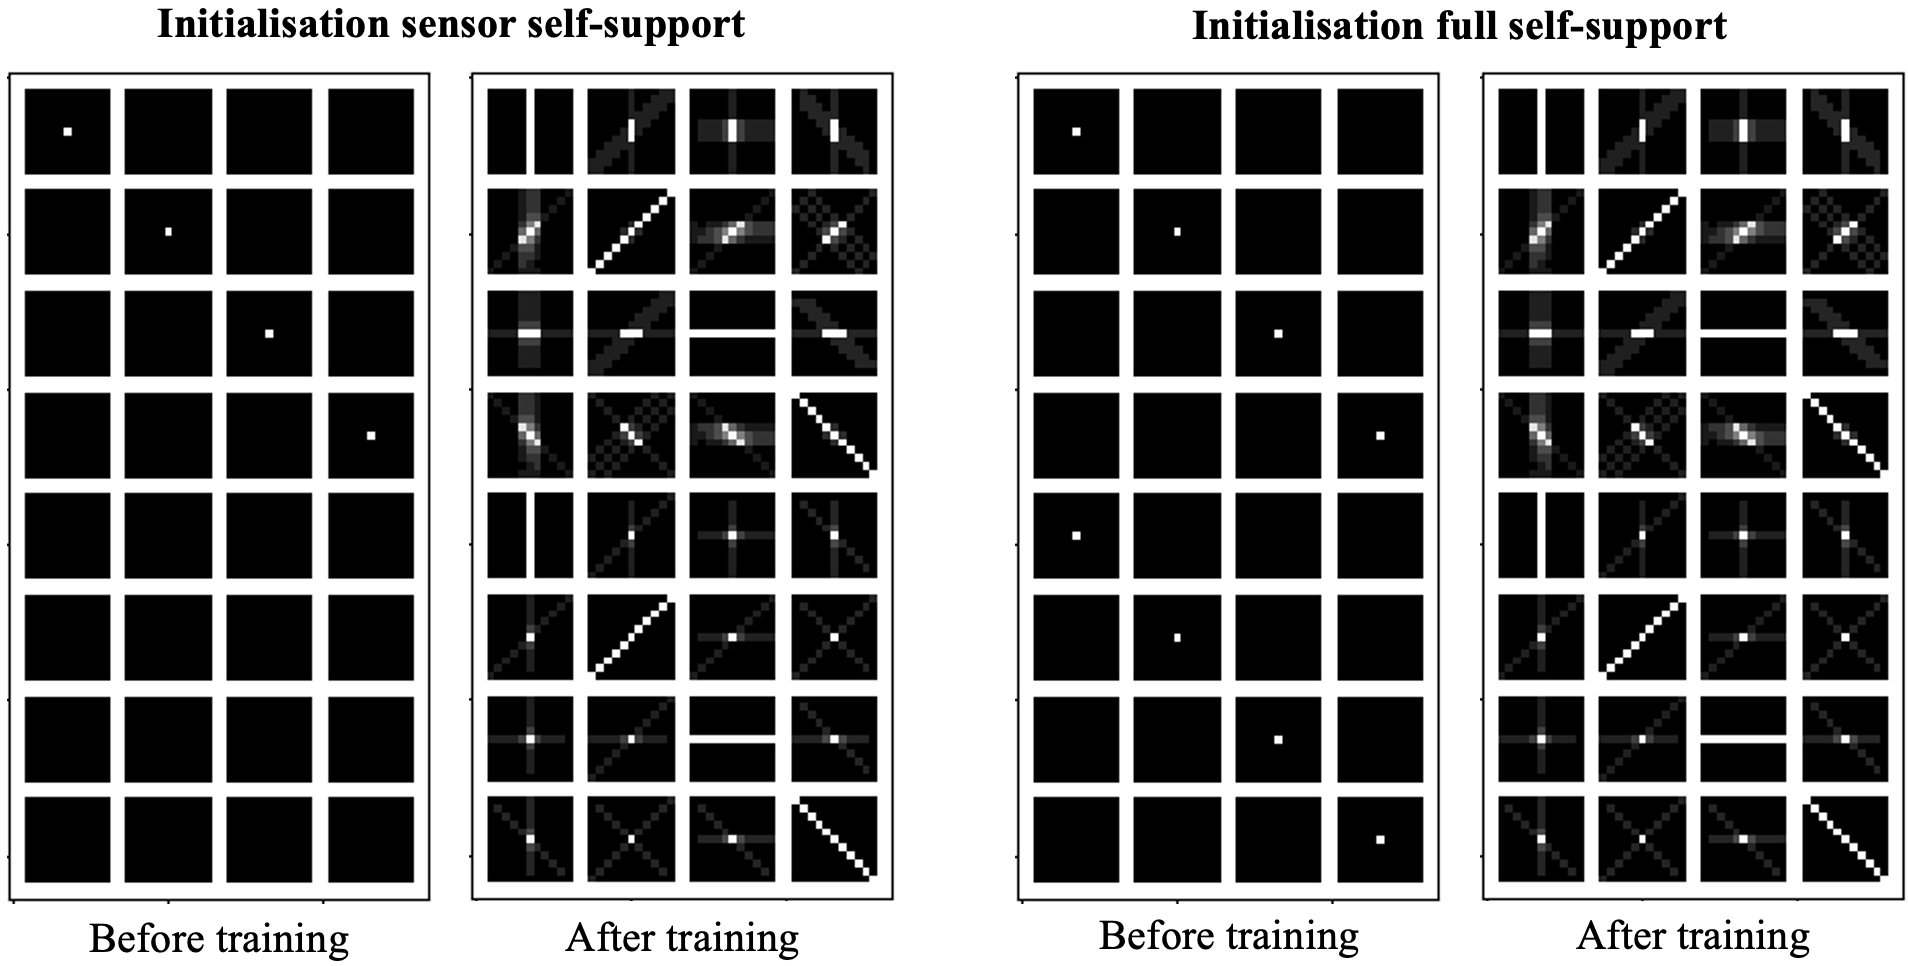
\includegraphics[width=0.99\textwidth]{init_weight_self_support}
    \caption[Weight initialisation with self-support]{Two different ways of initialising the weights of \emph{S1} with self support. For both initialisation strategies, the initial weights are shown on the left and the weights after training on the right.}
    \figlbl{init_weight_self_support}
\end{figure}

In this section, the crucial aspect of weight initialisation is discussed.
\secref{lateral_init} describes that initialising the weight with self-support is essential for the proper functioning of the network.
Two different approaches exist to initialise weights with self-support, as shown in \figref{init_weight_self_support}.
Regardless of the strategy chosen, both approaches lead to identical weight matrices after the training process.

\begin{figure}[h]
    \centering
    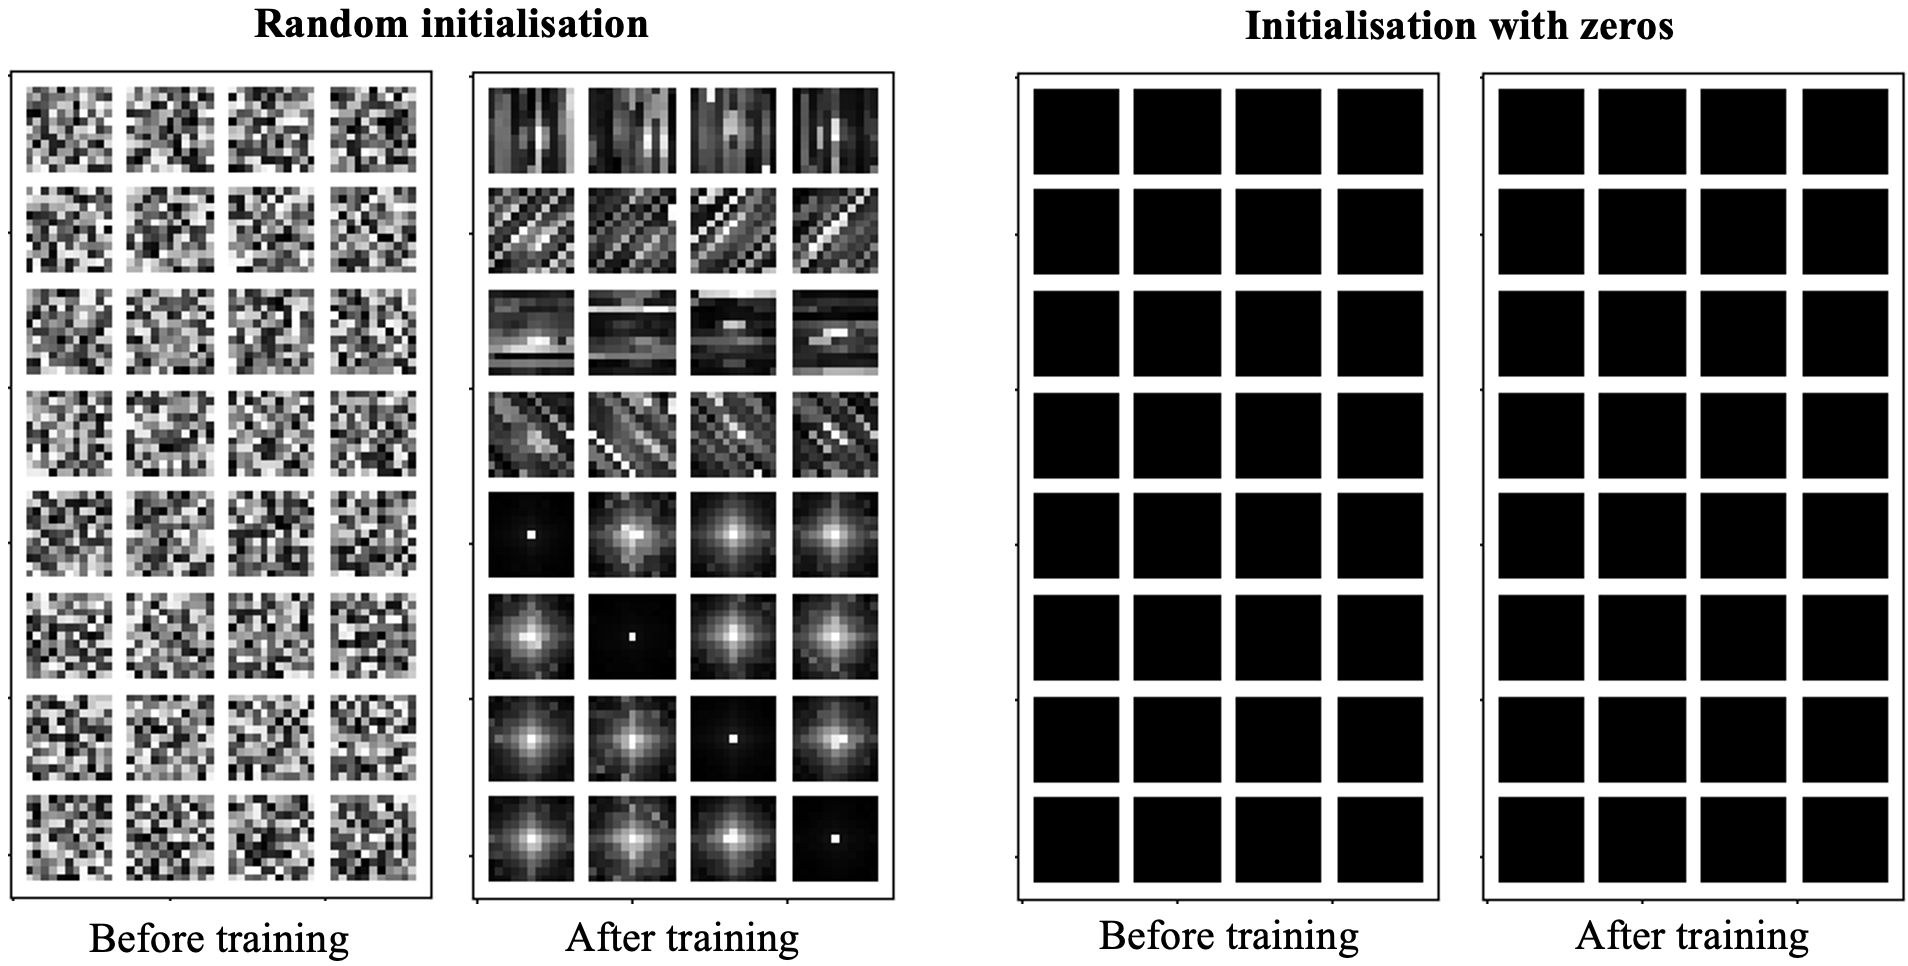
\includegraphics[width=0.99\textwidth]{init_weight_not_working}
    \caption[Random weight initialisation]{Two different ways of initialising the weights of \emph{S1}. The random weight initialisation strategy is shown on the left side of the image, and the zero initialisation strategy is shown on the right side. For both initialisation strategies, the initial weights are shown on the left and the weights after training on the right.}
    \figlbl{init_weight_not_working}
\end{figure}

However, it is important to note that not all weight initialisation strategies lead to good results. 
\figref{init_weight_not_working} show two other strategies and the resulting weight matrix after training:
Initialising the weights randomly leads to support between cells that should not support each other.
Consequently, this results in unwanted network activations, and the network converges towards weight parameters where the weights are almost identical across all output channels and do not provide lateral support in the desired manner.
If, on the other hand, the weights are initialised with zeros, the network has no active outputs. Consequently, all cells are immediately deactivated, and the weights remain unchanged during Hebbian learning.

In conclusion, using one of the two self-support weight initialisation strategies shown in \figref{init_weight_self_support} is crucial. These methods ensure proper functioning and effective learning, unlike the random or zero weight initialisation strategies depicted in \figref{init_weight_not_working}.

\section{Support Quality}
%
\begin{figure}[h]
    \centering
    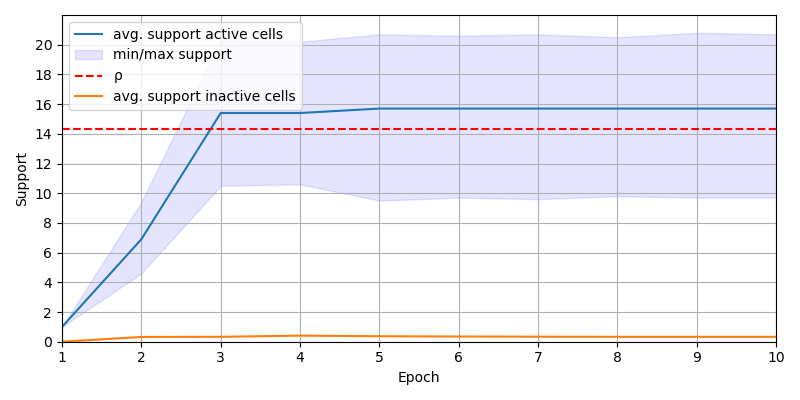
\includegraphics[width=0.99\textwidth]{support_strength}
    \caption[Average lateral support]{The average lateral support received by active and inactive cells during training. The y-axis shows the support, and the x-axis the training epoch. The blue line is the average, and the light blue interval is the min./max. support an active cell receives during training when no inhibition is used; the green interval represents the average/min./max. support an active cell receives support when inhibition is used; the orange line is the average support inactive cells receive. The dotted red line is the inhibition limit $\rho$, marking the threshold where the support is reduced.}
    \figlbl{support_strength}
\end{figure}
%
\figref{support_strength} presents the support strength received by active and inactive cells during training before the activation strength is normalised and translated into an activation probability.
The green interval depicts the support with inhibition and the blue interval without inhibition.

Before training, only self-support exists, i.e. the received support for active cells is $1$.
After training for $3$ epochs, the average support active cells receive increases to $13.8$ with inhibition and $15.7$ without inhibition.
At this point in training, most lateral connections have converged to a synaptic weight strength of $1$.
Thus, on average, a single cell is supported by approximately $14$ neighbouring cells.
On the other hand, inactive cells receive, on average, a lateral support of $0.3$, significantly less than active cells.
Thus, active cells receive much more lateral support after training, while inactive cells still do not receive significant support.
The support difference between active and inactive cells increases from $1$ at the beginning of training to $13.8$ after training.
This increase in support implies that it becomes much more difficult for individual cells to become active and explains why noise can be filtered efficiently.

The support active cells receive could increase further but is limited by the inhibitory strength $\rho = 1.3\cdot n_l = 14.3$.
When a cell exceeds this threshold $\rho$, its activation probability is linearly reduced.
This effect is visible when comparing the blue interval (without inhibition) with the green interval (with inhibition). The support strength for each cell is pushed below $\rho$, depicted as the red dotted line.

\figref{support_strength} show that cells can receive lateral support strengths of up to $21$ when no inhibitory signals are present in the network (see the max. values of the blue interval).
However, such strong support leads to undesired effects, as discussed in the next section.
When using an upper support limit $\rho$, the model tends to find a trade-off that only slightly surpasses this inhibition limit, thereby maximising the lateral support each cell receives while ensuring that each cell has a high activation probability.

The results depicted in \figref{support_strength} demonstrate that \emph{S1} builds net fragments as expected. The gap between the support strength of active and inactive cells becomes bigger during training, ensuring that only cells representing known patterns remain active.

\subsection{Inhibition}\seclbl{results_inhibition}
%
\begin{figure}[h]
    \centering
    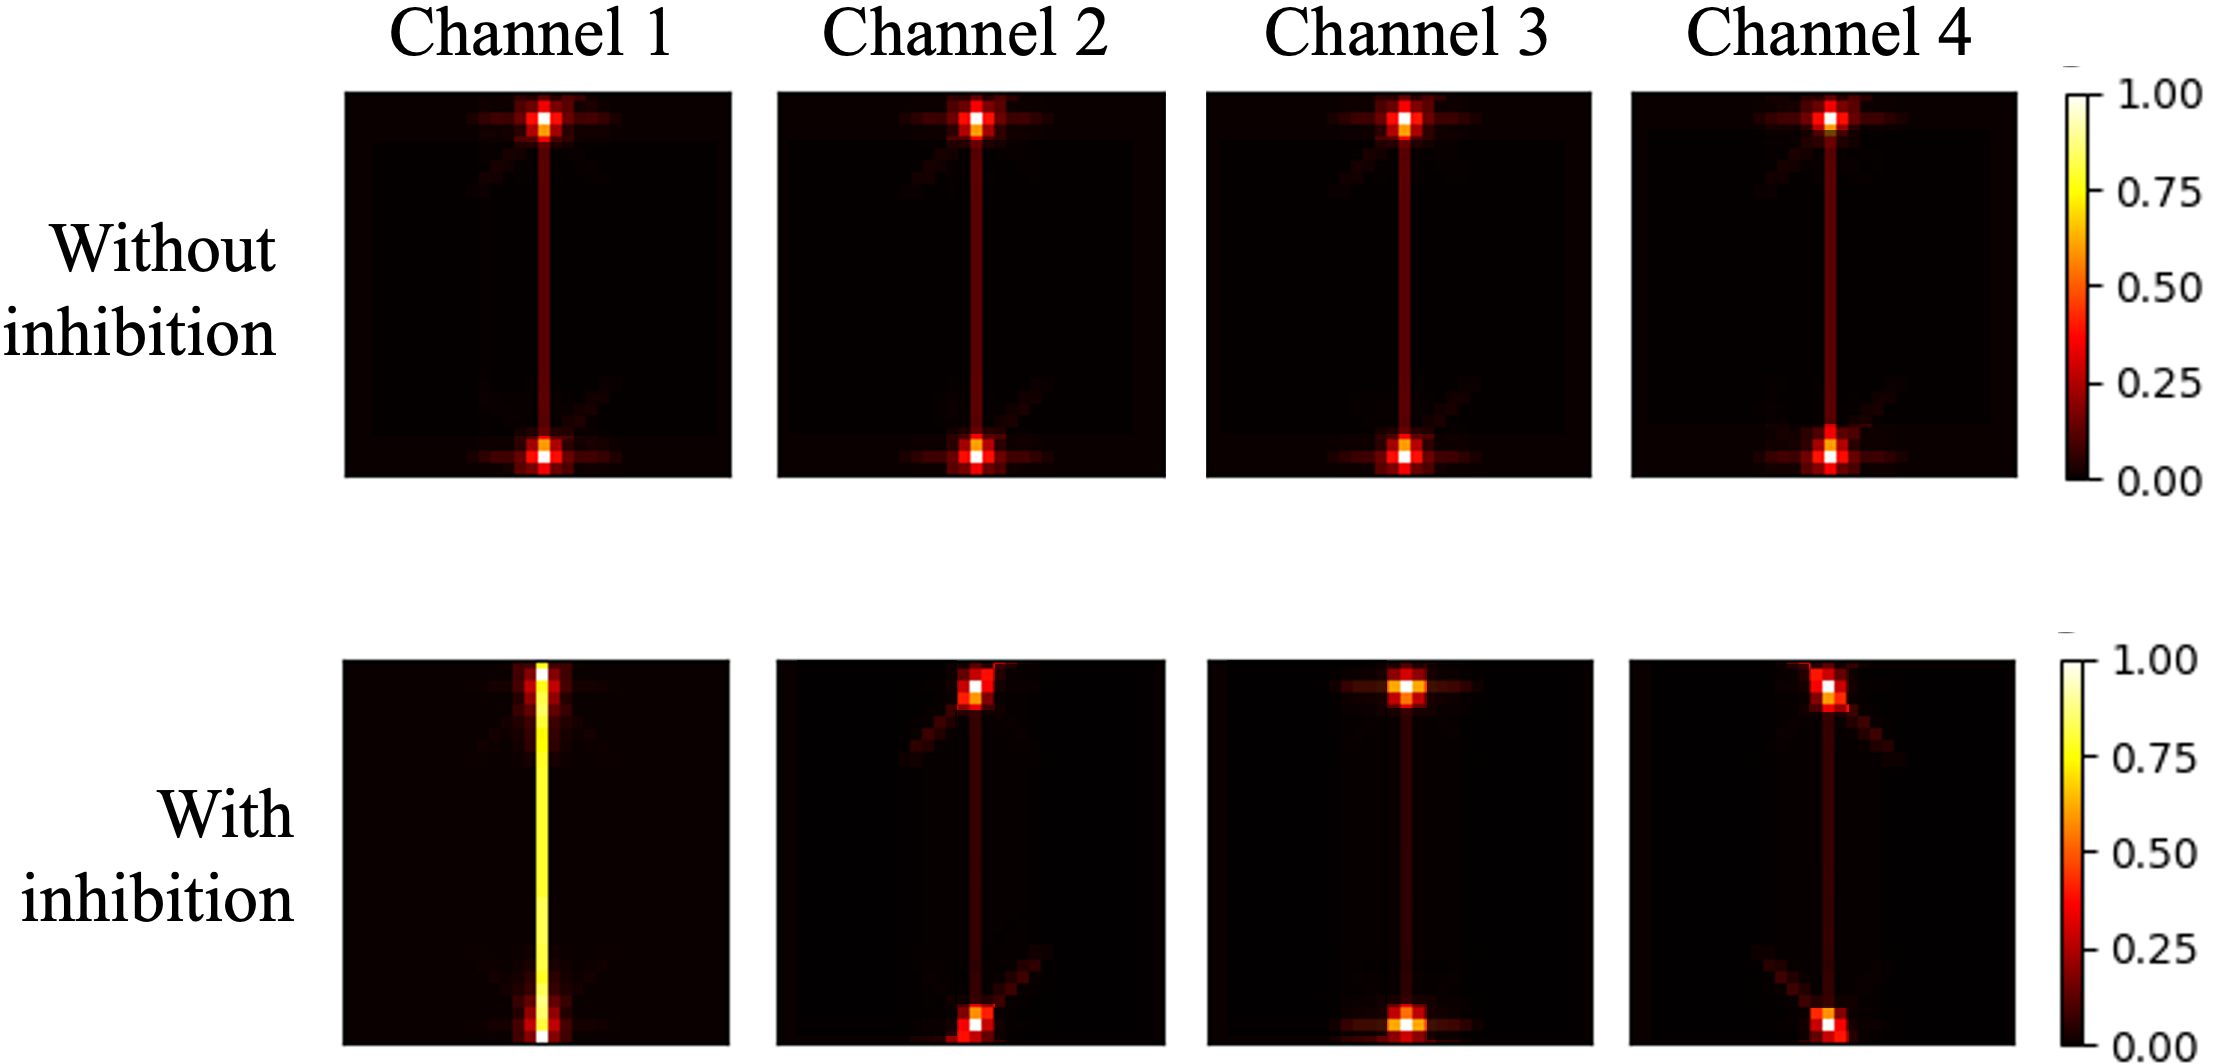
\includegraphics[width=0.79\textwidth]{inhibition_heatmap}
    \caption[Activation heatmap with/without inhibition]{The activation heatmap indicates the activation probability for all cells across the four channels. The upper row shows the probability without inhibition and the lower row with inhibition.}
    \figlbl{inhibition_heatmap}
\end{figure}
%
The following examines the impact of the inhibition threshold $\rho$. The activation heatmap shown in \figref{inhibition_heatmap} displays the activation probabilities for cells across four channels when a vertical line is fed into a model.
The top row shows the probabilities of a model trained without inhibition, while the bottom row shows the probabilities of a model trained with inhibition.

As discussed, all filters are active at the line ends, leading to many active cells and high lateral support in that region.
Specifically, the cell located at the line end receives lateral support from up to $21$ neighbouring cells if no inhibition is used.
When an activation strength of $21$ is mapped to an activation probability of $1.0$ and an activation strength of $0$ to $0.0$, the cells receive activation probabilities as visualised in the upper row of \figref{inhibition_heatmap}.
The pixels located at the line ends are dominant and have an activation probability of $1.0$, while the other pixels on the line have an activation probability of approximately $0.4$.
Therefore, only the cells at the line ends have a high activation probability but not the other cells depicting the middle of the line.

Introducing inhibition effectively addresses this issue.
With inhibition, the lateral support is limited to $\rho$.
The effect of inhibition on the activation probability per cell is shown in the second row of \figref{inhibition_heatmap}.
Notably, the activation probabilities of cells at the line ends remain high. However, the activation probabilities of the other pixels depicting the vertical line increase significantly, especially in the first channel, which represents vertical line features.

Please note that the two heatmaps in \figref{inhibition_heatmap} stem from different models.
Inhibition strongly influences the training process, and ``turning on'' inhibition would not convert the activation probabilities in the first into the ones shown in the second row.
Instead, inhibition normalises the activation probabilities throughout the training process, influencing weight updates.
Without inhibition, the activations are dominated by line ends, causing all channels to learn similar features.
With inhibition, the channels specialise more on distinct features as no feature dominates the learning process. Therefore, the weights (and thus the activation probabilities shown on the second row of \figref{inhibition_heatmap}) are more diverse.

\section{Conclusion}
The previous sections discuss the obtained results, thereby focusing on specific aspects.
In conclusion, \emph{S1} can build net fragments, and it is demonstrated that these fragments associate input patterns with learned patterns, thereby removing noise or reconstructing occluded parts of objects.
Since removing noise and reconstructing objects improves representations over multiple timesteps, it is considered a hierarchical processing of features without being subject to early commitment.
Thus, the experiments demonstrate that net fragments can be implemented according to the proposed principles.

This is considered an important step towards implementing the proposed framework.
Implementing projection fibres is based on the principle of comparing local features in \emph{S1} and \emph{S2} and initiating a mapping between them if neighbouring fibres agree \sidecite{bienenstock_neural_1987, lades_distortion_1993, wiskott_face_1996}.
Such a mapping only works well if patterns in the two stages are highly similar.
This is achieved with net fragments that either turn off cells representing unknown patterns that are not present in \emph{S2} and thus cannot be mapped or support and reconstruct (i.e. optimise) existing patterns to become more similar to patterns stored in \emph{S2}.
Thus, the conducted experiments lay the foundation for future research and implementing projection fibres that map net fragments instead of cells as done in previous work (c.f. \secref{projection_fibres}).